\section{Diagramas de caja}
Se construyen diagramas de caja con los 485 meses completos entre enero de 1981 y diciembre de 2022. Los 19 meses con algún día faltante se excluyen; no se reemplazan por cero. P, Q y R no tienen meses válidos con valor cero. Para temperatura, un valor de 0~$^\circ$C se consideraría una observación válida y nunca una ausencia.

P presenta media y mediana muy próximas (168,20 y 168,47~mm), pero un rango amplio. Q y R muestran media mayor que mediana (98,70 frente a 85,55~m$^3$/s; 92,82 frente a 81,40~mm), consistente con asimetría hacia valores altos y con crecientes poco frecuentes. Los puntos fuera de 1,5 veces el IQR no se eliminan: deben revisarse en las cronologías y, cuando sea posible, contra los datos diarios y metadatos. Las cajas de temperatura son mucho más compactas que las de P, Q y R.

\begin{figure}[H]\centering
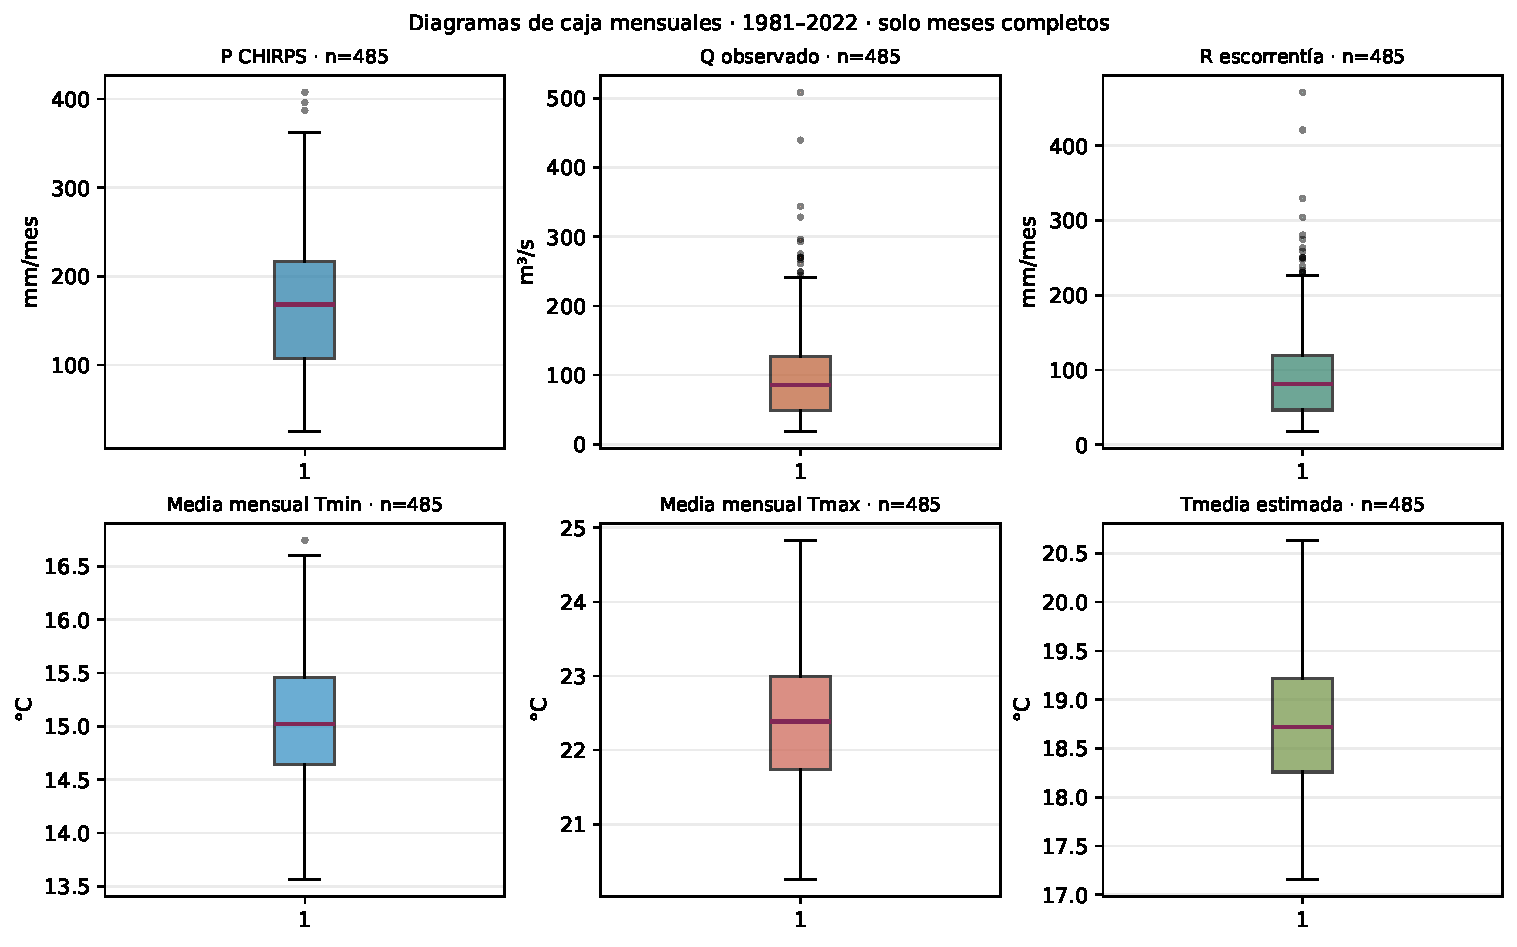
\includegraphics[width=\linewidth]{figuras/diagramas_caja.pdf}
\caption{Diagramas de caja de meses válidos. La línea central es la mediana; la caja representa Q1--Q3; los puntos son valores fuera de 1,5 IQR.}
\end{figure}
